
\myNewSlide
\section*{Frequentist hypothesis testing: coin flipping example}
$N=100$ and $h=60$\\
Can we reject the fair coin hypothesis? $H_0:\Pr(\mbox{heads}) = 0.5$

The ``recipe'' is:
\begin{compactenum}
    \item Formulate null ($H_0$) and alternative ($H_A$) hypotheses.
    \item Choose an acceptable Type-I error rate (significance level)
    \item Choose a test statistic: $f_H$= fraction of heads in sample. $f_H=0.6$
    \item Characterize the null distribution of the test statistic 
    \item Calculate the $P$-value: The probability of a test statistic value more extreme than $f_H$ arising {\em even if $H_0$  is true}.
    \item Reject $H_0$ if $P$-value is $\leq$ your Type I error rate.
\end{compactenum}

\myNewSlide
\begin{picture}(500,0)(0,0)
      \put(0,-190){\makebox(0,0)[l]{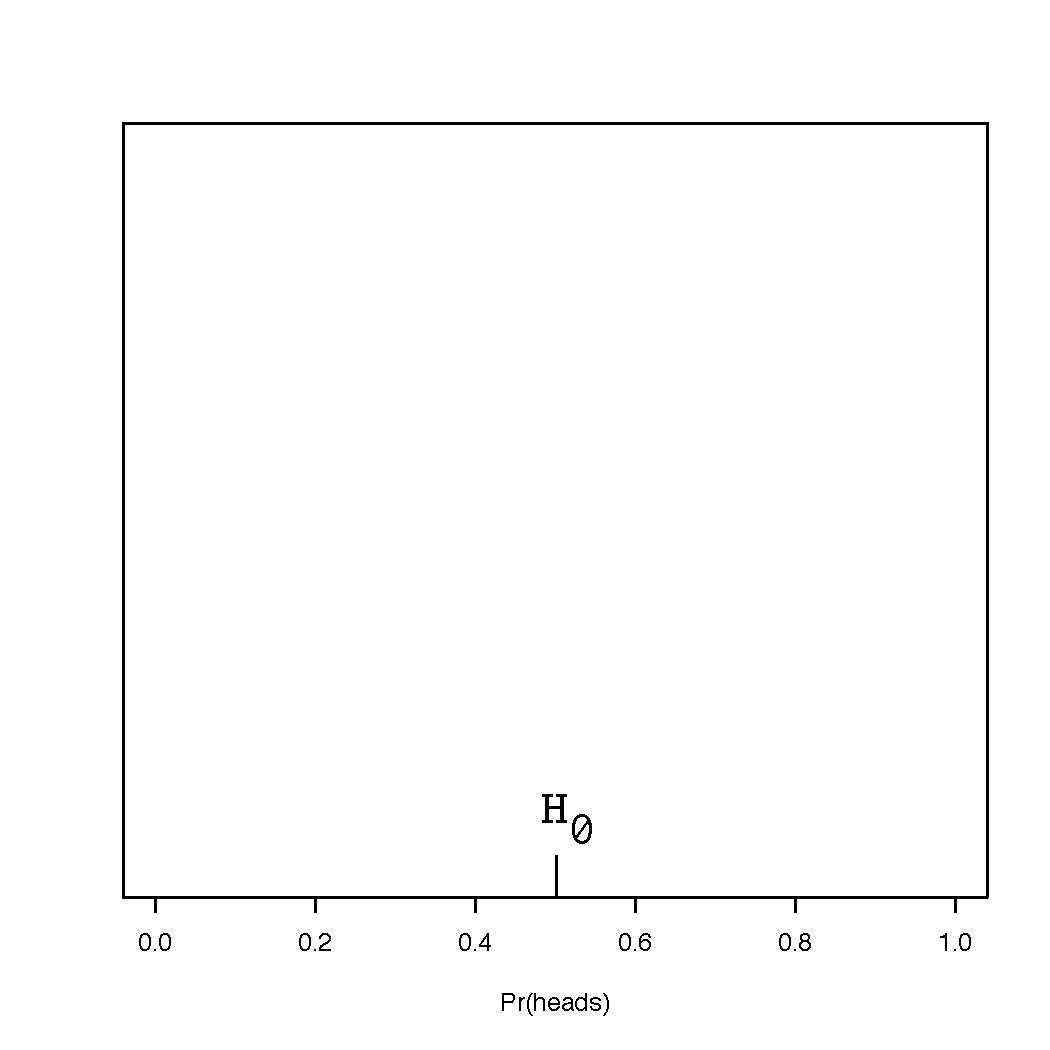
\includegraphics[scale=1.0]{../newimages/coin_axes.pdf}}}
\end{picture}

\myNewSlide
\begin{picture}(500,0)(0,0)
      \put(0,-190){\makebox(0,0)[l]{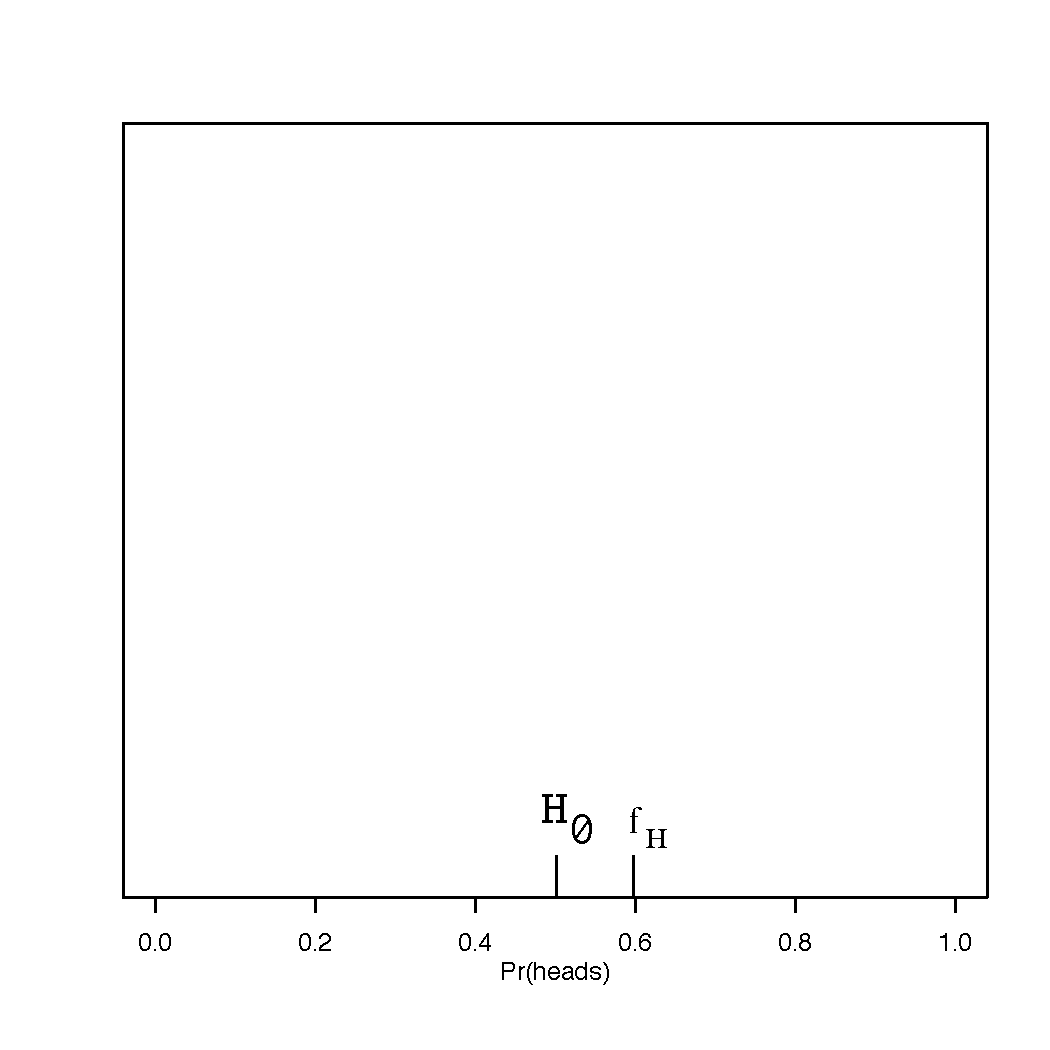
\includegraphics[scale=1.0]{../newimages/coin_axes_data.pdf}}}
\end{picture}

\myNewSlide
\section*{Null distribution}
\begin{picture}(500,0)(0,0)
      \put(0,-190){\makebox(0,0)[l]{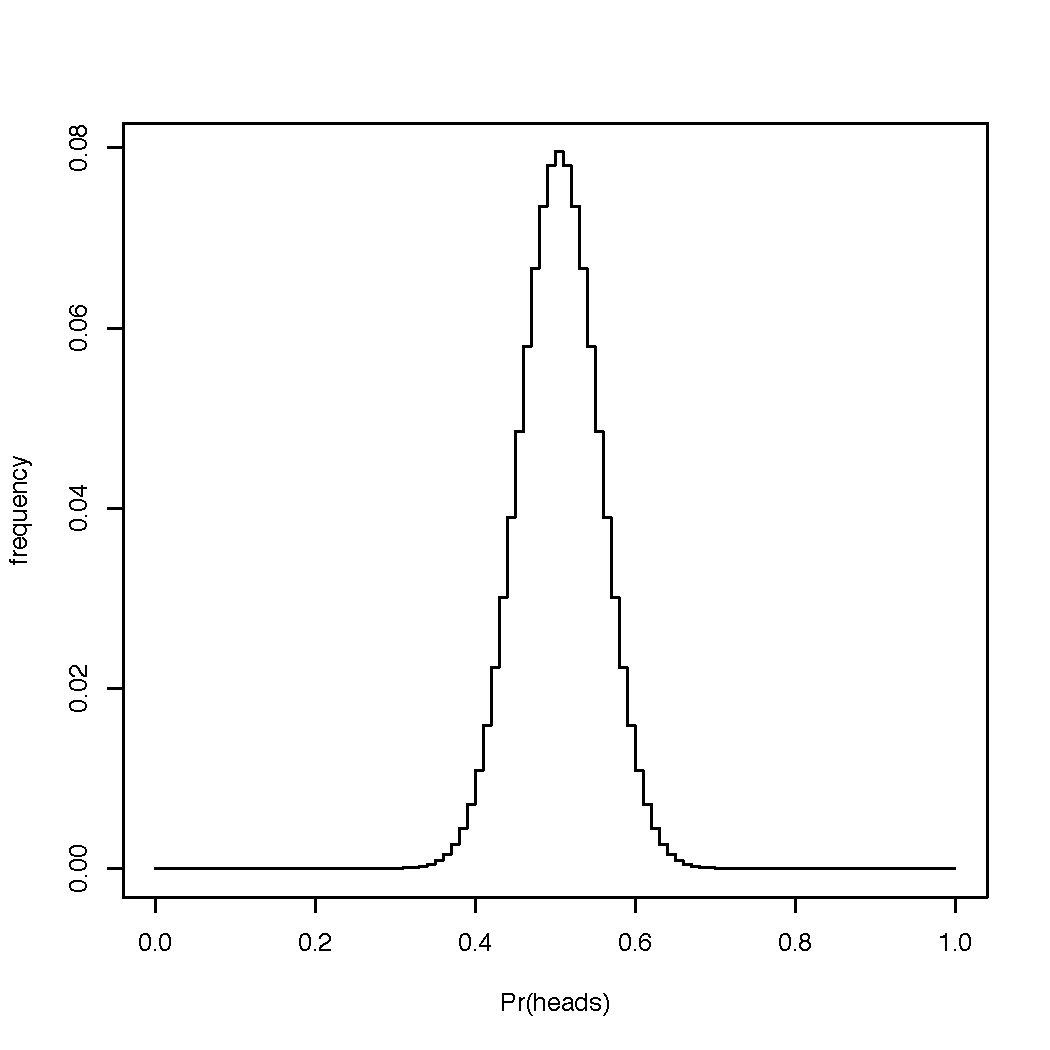
\includegraphics[scale=1.0]{../newimages/coin_wo_tails.pdf}}}
\end{picture}

\myNewSlide
\begin{picture}(500,0)(0,0)
      \put(0,-190){\makebox(0,0)[l]{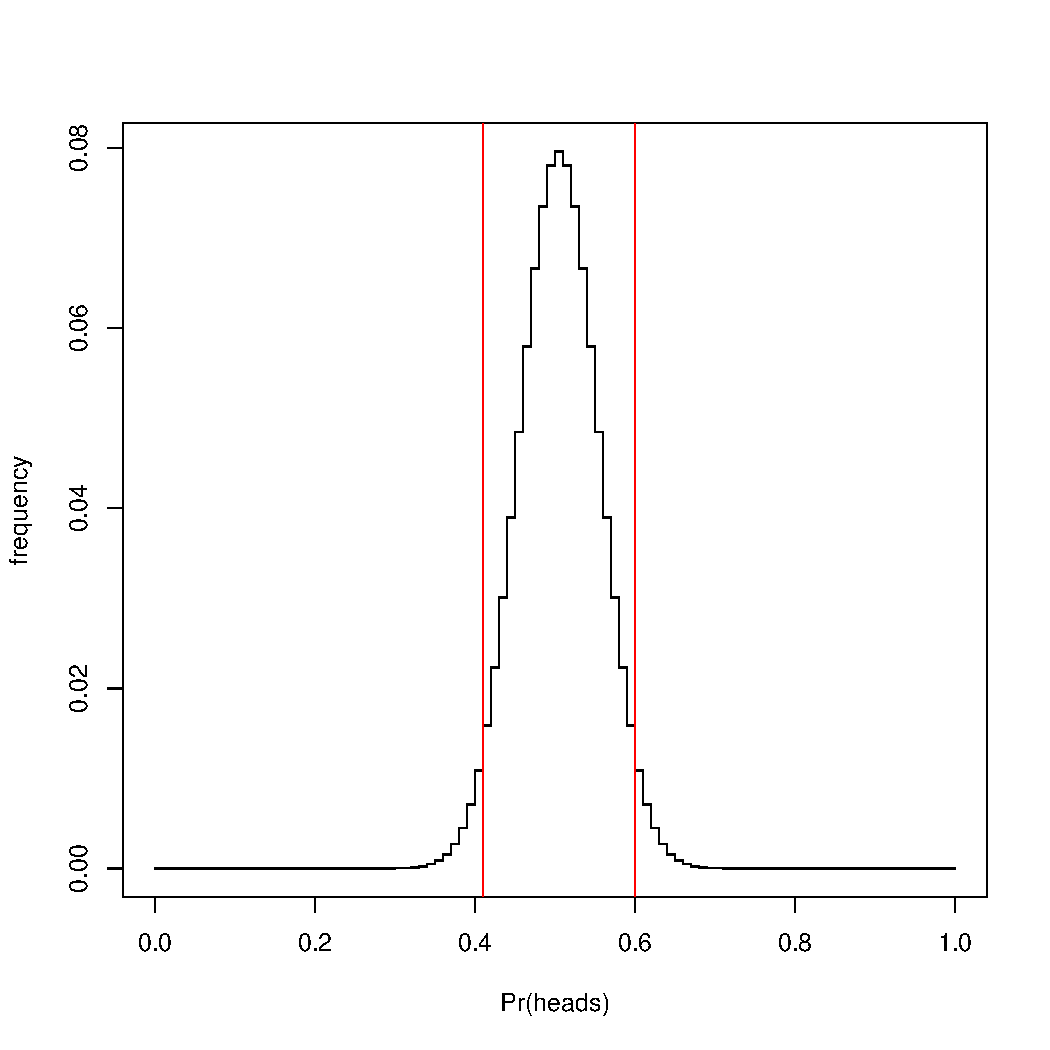
\includegraphics[scale=1.0]{../newimages/coin_w_tails.pdf}}}
      \put(0,-450){$P$-value $\approx$ 0.058}
\end{picture}

\myNewSlide
Making similar plots for tree inference is hard.

\begin{itemize}
    \item Our parameter space is trees and branch lengths.
    \item Our data is a matrix of characters.
    \item It is hard to put these objects on the same. 
    You can do this ``pattern frequency space''. Some projections of this space are:

\end{itemize}


